\subsection{Molecular Dynamics}
\paragraph{}
Due to the size of biological systems, current computational power is unable to simulate every atom within an enzyme at a true \gls{acr:QM} level and so some approximations must be made in order to simplify the system. The traditional method for simulating large biological molecules such as enzymes is to use a classical physics (\gls{acr:MM}) approach (Equation: \ref{eq:EMM}), which includes using empirical force fields derived from classical physics in order to describe the system. The use of classical physics allows for much simpler calculations and so increases computational efficiency dramatically, allowing us to simulate millions of atoms in a relatively short time scale. 

\begin{equation}
\label{eq:EMM}
\begin{split}
E_{Total} & = E_{Bonded} + E_{Non-Bonded} \\
E_{Bonded} & = E_{Bond} + E_{Angle} + E_{Dihedral} \\
E_{Non-Bonded} & = E_{Electrostatic} + E_{van ~der ~Waals} \\
\end{split}
\end{equation}

\paragraph{}
Molecular mechanics requires empirical forcefields\cite{Ponder2003ForceSimulations} to describe the behaviours of different atoms (and more importantly biological residues) to describe the energies of the different interactions within a system and so selecting a suitable forcefield which has been parametrised for your use case is important for achieving accurate results. For enzymes, the two most commonly used forcefields are CHARMM\cite{Vanommeslaeghe2009CHARMMFields} and AMBER\cite{Maier2015Ff14SB:Ff99SB} which were both parametrised for proteins and nucleic acids. 

\begin{figure}[H]
    \centering
    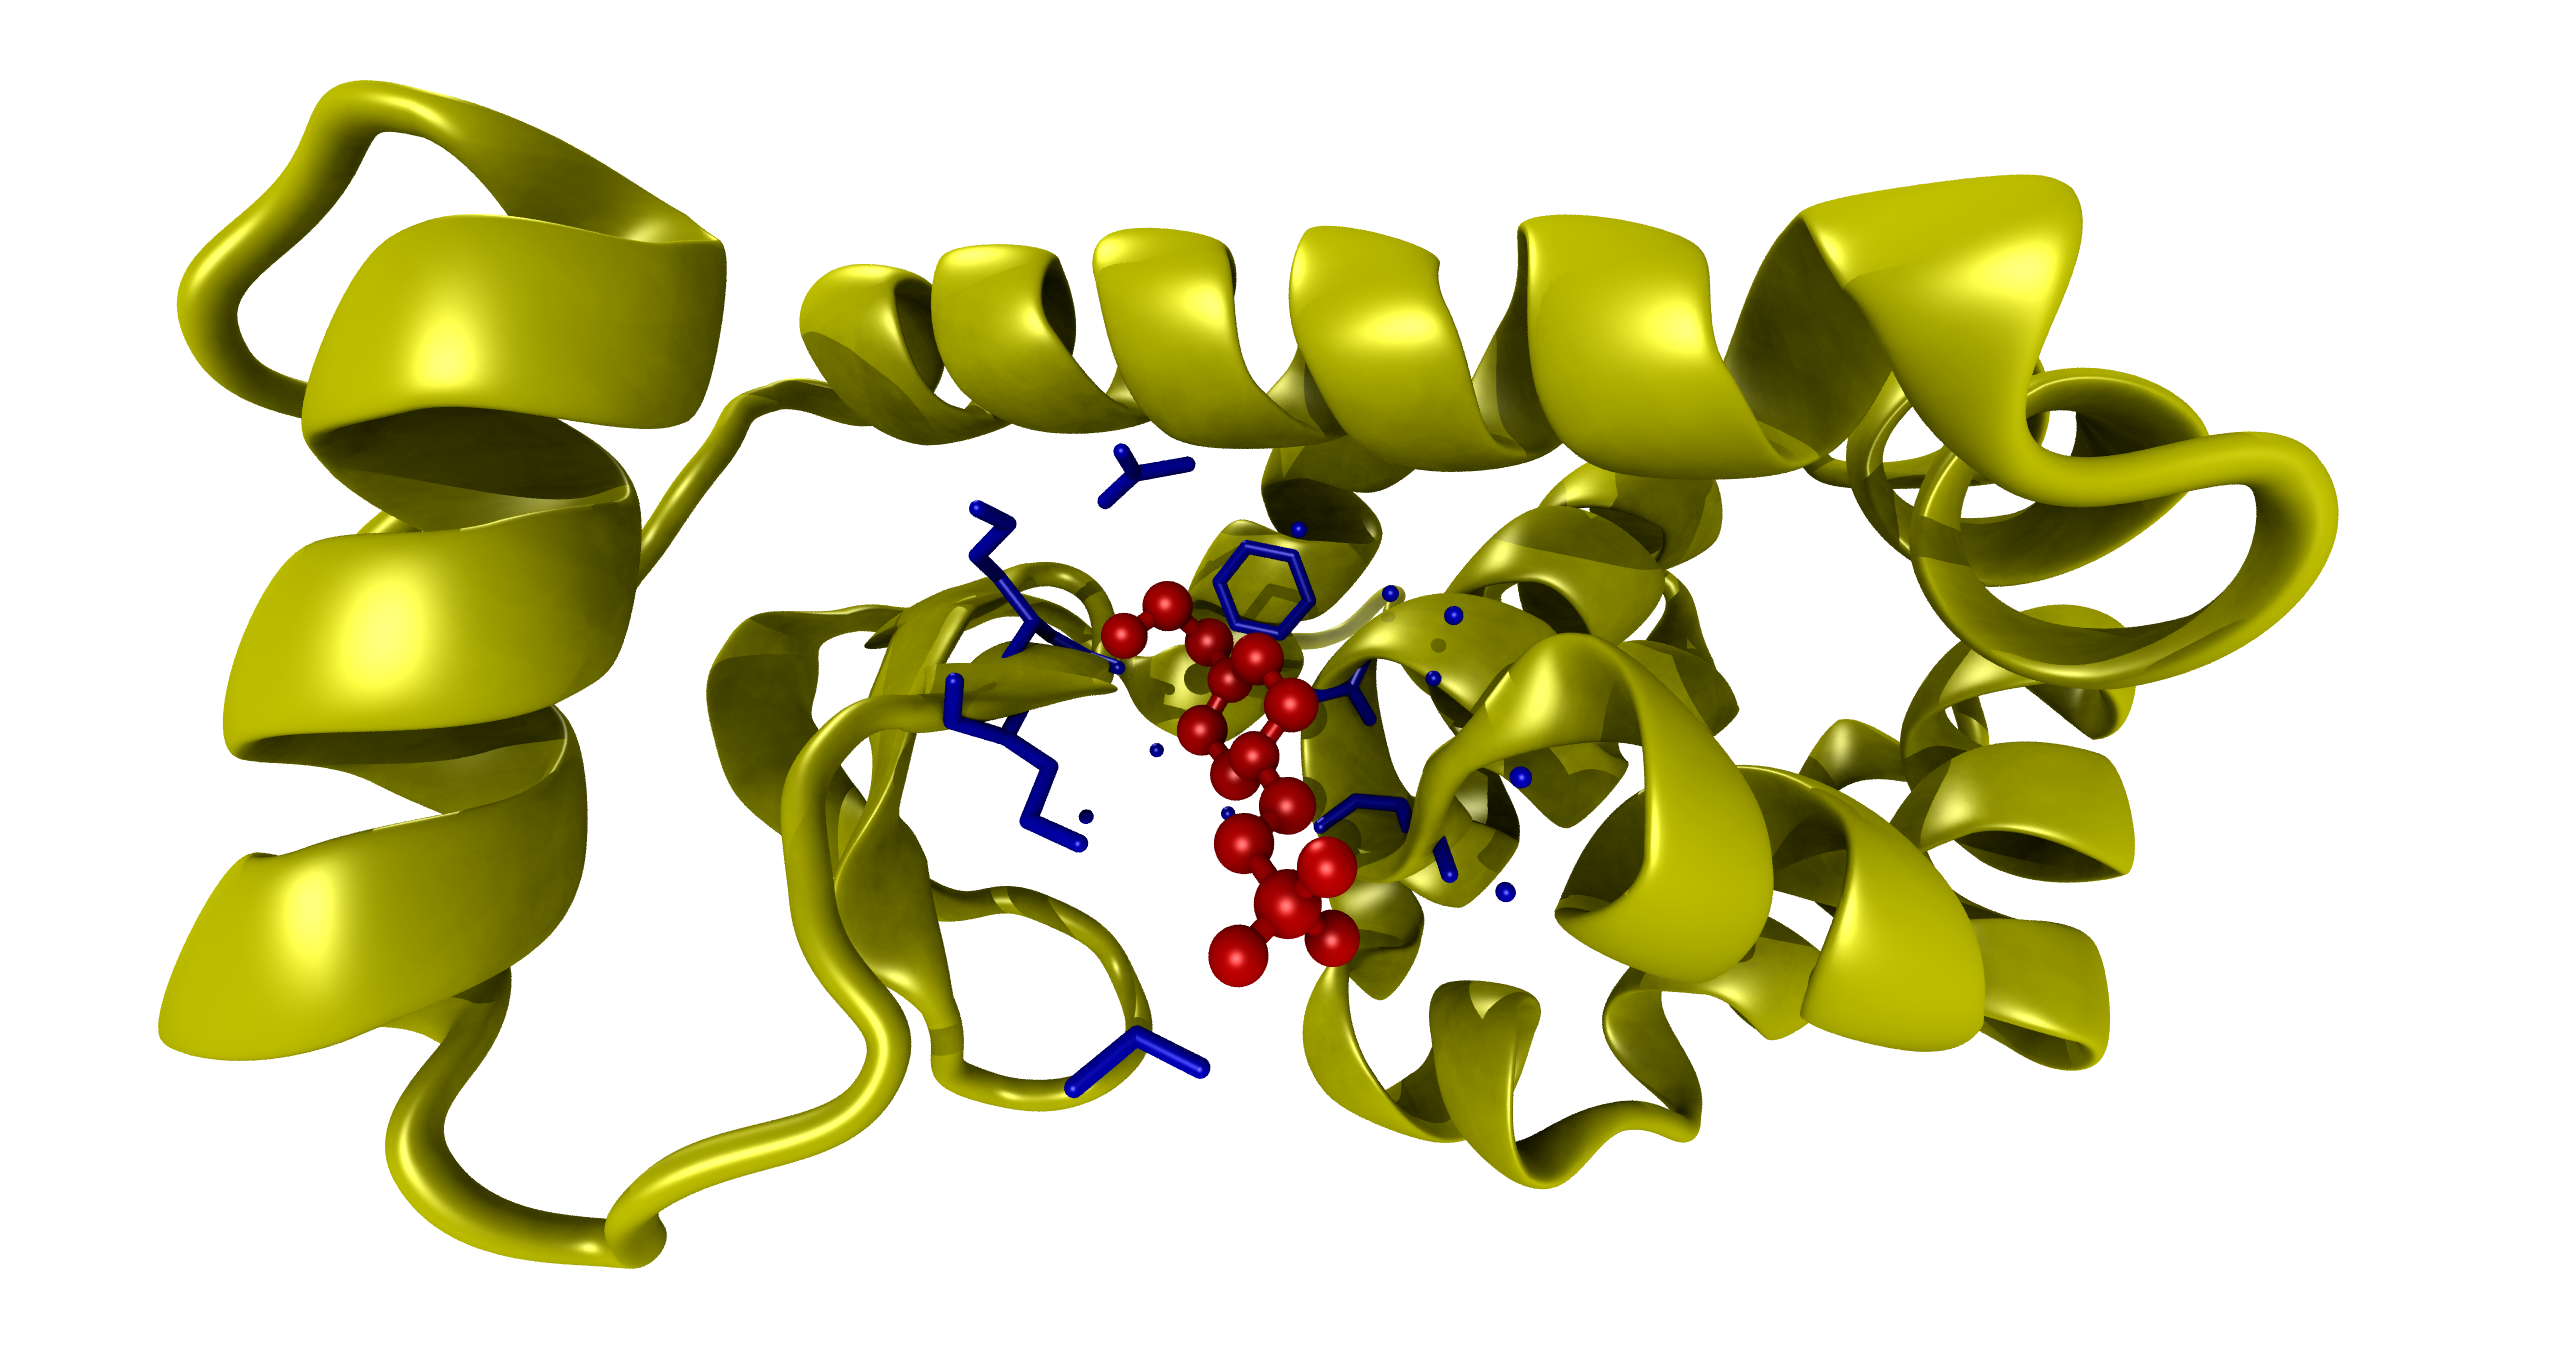
\includegraphics[width=\textwidth]{Graphics/Theory/QMMM.png}
    \caption{A visual representation of a QM/MM calculation where the atoms in yellow are treated at the \gls{acr:MM} level of theory, the atoms in red are treated at the \gls{acr:QM} level and the atoms in blue are treated at both levels of theory.}
    \label{fig:QMMM}
\end{figure}

\paragraph{}
These \gls{acr:MM} methods can be combined with QM methods in order to calculate the reaction center with high accuracy \gls{acr:QM} theory whilst also including interactions with the wider environment, specifically the electrostatic, dispersion and structural effects, which can control the structure of the reaction site and the thermodynamics of the system. In \gls{acr:QM}/\gls{acr:MM} you split the system into two or three sections (usually three) with your reaction site and any atoms which are known to be directly involved being put into the \gls{acr:QM} region. Then a thin layer around this region is included  as a hybrid zone which allows for communication between the two methods and used when the zone boundary intersects a covalent chemical bond. These atoms are usually calculated at both levels of theory. Finally the rest of the system is treated at the simplest level of theory (\gls{acr:MM}) (Figure: \ref{fig:QMMM}).